\documentclass[10pt,twocolumn,pdftex]{article}
\usepackage[margin=1in]{geometry}
\usepackage{comment}
\usepackage{graphicx}
\usepackage{url}
\usepackage[pdftex,colorlinks=true,citecolor=black,filecolor=black,%
            linkcolor=black,urlcolor=black]{hyperref}
\usepackage{times}
%\usepackage{listings}
%\usepackage{fancyvrb}
%\usepackage{amsmath}
%\usepackage{amsthm}
%\usepackage{amssymb}

%\lstset{ % for our code environment
%    language={},
%    basicstyle=\ttfamily}
%\let\code\lstinline

\title{Title of Paper}
\author{Student Name \\
\url{student.name@email.wm.edu}}
\date{}

\begin{document}

\maketitle

\begin{abstract}
  %Abstract here \ldots Remember to talk about the area, problem,
  %solution, methodology, results, and take-away. In general, an abstract
  %should only be one paragraph and on the order of 200 words.

  Analyzing Android applications for correct security practices such as using permissions, using the SSL API, and potential interface vulnerabilities 
  is a challenging task. This paper presents our tool CRAB-Droid, a python script that builds upon Androguard to carry out a static analysis to identify potential security vulnerabilities in Android applications.
  We analyzed 100 apps from the Google Play Store with the objective of identifying potential security vulnerabilities. We created 5 experiments to test on our 7 research questions we had outlined in the planning stage 
  of our analysis. Our findings ... \#TODO This project shows the significance of developers following best practices when creating Android apps, and the abilities to develop tools to help guide and educate 
  engineers to them. Implementing tools like Androguard and CRAB-Droid to be used in the development process can help to identify potential security vulnerabilities before putting apps into deployment onto the app stores.
  This can help to save time, money, and most of all, user privacy. 
  
\end{abstract}

\section{Introduction}

% The Introduction includes references to highly-relevant related work,
% i.e., state of the art for the problem you are trying to solve.

% Note: when writing \LaTeX, each paragraph should have a line separated
% between it and the separate paragraph. This causes proper indentation
% and makes the document more readable. Do not end paragraphs with
% \verb/\\/.

% The remainder of this paper proceeds as follows.
% Section~\ref{sec:overview} overviews our sample paper.
% Section~\ref{sec:design} describes the design of our sample paper.
% Section~\ref{sec:eval} evaluates our solution.
% Section~\ref{sec:discussion} discusses additional topics.
% Section~\ref{sec:relwork} describes related work. Section~\ref{sec:conc}
% concludes.

Currently, Android is the most used smartphone operating system in the world, with a market share of 48\% and over 400,000 applications (apps) available in the Google Play Market \cite{10.1145/2382196.2382205}. The Google Play
Market is also mostly open and unrestricted, allotting developers more freedom, but many times at the cost of security. 
The ability to identify vulnerablities within Android applications is vital to the safety of users and their information. Showcasing these vulnerabilities then
helps to educate developers to carry-out best security practices when creating an app and to take vulnerable apps off the app store to be secured. This project investigates a variety of Android applications and vulnerabilities that potentially 
exist within them. 

With technological enhancements to smartphone devices over the past two decades, users have been downloading more and more apps to their phones. This rise of phone apps results in a greater chance for users to download malicious ones 
that may contain malware, such as trojans \cite{10.1145/1653662.1653691}. This spike has also lead to many new developers entering the ever expanding market, with many potential bad security practices in apps along with them. For reasons mentioned previously, 
it is important to identify these vulnerabilities in order to educate developers and protect users. 

For this project, we analyzed a set of 100 Android apps from the Google Play Store. We then established seven research questions to hypothesize about pontential vulnerabilites we believed we would find in the apps. We organized them into three domains: permission misuse, 
SSL API misue, and interface vulnerabilites. These domains were chosen to cover a broad attack vector of the Android applications such as the use of permissions that may violate user privacy, the use of SSL APIs that may not be secure, and the use of interfaces that may be vulnerable to attacks.
Five experiments were then developed and tested on our set of apps. 

The five experiments were tested on each app as follows: test apps for whether they use all the permissions they request and if they use any dangerous permission combinations, examine for overridden trust manager and error handler methods, 
test for implementation of the AllowAllHostnameVerifier class, see if apps contain mixed use of HTTP and HTTPS (mixed SSL), and finally test apps for incorrect use of the addJavascriptInterface method.

Using the Androguard library \cite{androguard} and referencing Mallodroid \cite{10.1145/2382196.2382205}, we completed a thorough analysis of the apps. The results showed ... %TODO add results

Overall, the significance of this project is seen in its use of static analysis and its applications in the discipline of Android mobile app security. This practice has the potential to be utilized in real-world applications to help secure the Google Play Store and protect users from malicious apps. 

\section{Methodology}
\label{sec:overview}

Overview of Approach (a nice and accessible ``English'' description of
your approach). Don't forget a niche high-level figure. Our sample
high-level figure is shown in Figure~\ref{fig:overview}.

There is sometimes a background section before the overview section. In
general, you want to try to get your high level figure somewhere between
pages 2 and 4. It is generally bad to have a figure on the first page
(but was unavoidable in this sample).

% You may need to move this \begin{figure} ... \end{figure} block around
% in the document to place it in a logical spot in the paper. In
% general, get the figure on the same page as the prose that refers to
% it.
\begin{figure}[t]
  \centering
  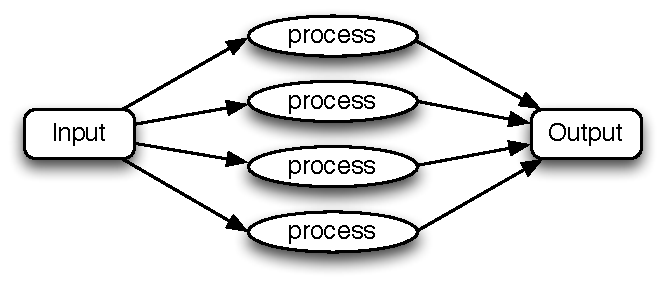
\includegraphics[width=3in]{figs/overview}
  \caption{A high-level architecture of our approach}
  \label{fig:overview}
\end{figure}

\section{Design}
\label{sec:design}

Protocol/Architecture/Design/\ldots

\section{Evaluation}
\label{sec:eval}
%Evaluation (don't forget to interpret your data)

This section comprehensively evaluates the performance of our proposed and tested experiments. It determines which experiements performed the best on criteria of 
most true positive matches and least false positive matches. 

\section{Discussion}
\label{sec:discussion}

Discussion (discuss some of the important simplifying assumptions, and
suggest possibilities for future work)

\section{Findings}
\label{sec:relwork}

Related Work (``somewhat related'' work goes here; directly related work
goes into the Introduction)~\cite{dsd13}.

\section{Conclusion}
\label{sec:conc}

%Conclusions (don't summarize your work here. That's what the abstract
%was for. Instead provide some philosophical ruminations of your work and
%future possibilities, i.e., conclusions that you have arrived at as a
%result of your work.)



\bibliographystyle{abbrv}
\bibliography{main}

\end{document}


